\section{Results}
\label{sec:results}

This section reports what the typed contracts, the training recipe and scale deliver, what a decision
costs, and two controlled experiments on how inputs are rendered. All checkpoints share the architecture
fixed in \Cref{sec:analysis}.

\subsection{Typed output contracts}
\label{sec:results:typed}

\textbf{Each output type delivers the property its contract names, with backbone, tap and readout
fixed.} We compare matched fine-tunes from one parent checkpoint, each trained for 3k steps on the rows
of its own type, against a control that treats the same rows as plain Choice; full tables are in
\Cref{app:typed-primitives}.

\textbf{Score.} The ordinal-smoothed target ($\tauord = 0.7$) adds no parameters and improves every
probability-quality measure on held-out urgency at flat accuracy (.505 $\to$ .508): NLL 2.07 $\to$ 1.23,
Brier .79 $\to$ .68, ECE .35 $\to$ .19, ordinal MAE .58 $\to$ .55. On JevBench's 12 ordinal items the
two models make identical per-item predictions, so the gain is in how mass is spread over adjacent
levels. On an external severity set it also lifts accuracy from .853 to .939 and cuts MAE from .15 to .06.

\textbf{Noul.} The Bernoulli head renders no candidates, so label order cannot enter its computation.
Reversing the labels of a two-way Choice over \{no, yes\} moves $P(\text{yes})$ by up to .55 (mean
.01--.15 across sets); the Bernoulli head moves it by exactly zero on all nine test sets. It is better or
equal on six of seven yes/no sets and clears the untouched PagerDuty floor by a wide margin: accuracy
.602 $\to$ .886 against a .792 majority floor, NLL 1.04 $\to$ .28. Only rows whose candidate set is
exactly \{yes, no\} take the Bernoulli path.

\subsection{The training distribution}
\label{sec:results:mixture}

\textbf{Decision-type balance, counterfactual rubric groups and null targets each move a separate axis.}
All comparisons here are matched 1.7B runs that differ only in data or sampler.

\textbf{Family balance.} Adding workflow data at family weights E .35 / K .25 / W .40 cost 11 points on
CLINC-150 and 10 on TREC-fine, almost all of it false abstention (CLINC-150 .05 $\to$ .17). In a sweep of
the evidence share (\Cref{tab:app-mixture}), $E \ge .45$ brings NLI and BoolQ back within 1 point of the
evidence-only base and intent and topic sets within 3--4, with workflow metrics unchanged within 1--4.

\textbf{Counterfactual rubric groups.} DecisionMix v2 places every training row in a group that shares
a state and candidate set across rubrics with different gold answers (\Cref{sec:train:rubric}). Added
together with the uncertainty corpus, against a control never trained on either, it lifts held-out
families, grammars and rubric styles from .481/.507/.491 to .827/.881/.888, and accuracy on held-out
rubric-flip pairs from .477 to .710. Accuracy under a shuffled rubric falls from .446 to .405: the model
now depends on the rubric it is given. Level-7 composition, which the generator never produces, moves
from .477 to .498 (\Cref{sec:limitations}). The original workflow sets give up 3--5 points at a fixed
workflow share now split over four corpora.

\textbf{Null augmentation.} Duplicating 20\% of workflow rows with the gold candidate removed and target
$\nullsym$ lowers false abstention on CLINC-150 from .10 to .08 and on TREC-fine from .27 to .12, and
raises accuracy by 2.6, 3.6, 4.3 and 6.0 points on CLINC-150, TREC-fine, HWU64 and 20NG. MMLU-Pro
among-$\numcands$ returns to the evidence-only base (.353), with the highest $\dqsh$ of any mixture
(.143). The model now spends mass on $\nullsym$ where soft gold has none, so held-out Noul drops 4 points
and soft-target NLL rises. Any augmentation fraction in [.10, .20] gives the same model within noise.

\textbf{Soft targets.} The uncertainty corpus, added in the same run, trades top-1 accuracy for
likelihood (ChaosNLI NLL 1.27 $\to$ 1.00 with accuracy .584 $\to$ .537), and typed-decisions NLL improves
from 2.06 to 1.71.

\subsection{Probability quality}
\label{sec:results:calibration}

\textbf{Probability quality is indexed by decision type, so it is set by training and checkpoint
selection.} One global temperature and null-logit offset, fit jointly on held-out soft-target rows,
wants opposite corrections for two checkpoints. For an evidence-and-knowledge checkpoint the fitted
offset is $-1.75$, which cuts CLINC-150 false abstention from .053 to .022. For a workflow-trained
checkpoint it is $+3.0$, which repairs typed-decisions NLL (1.95 $\to$ 1.19) and held-out Score NLL
(2.03 $\to$ 1.09) and collapses intent and topic coverage to 5--9\%. Null augmentation and per-type
targets supply the correction at the level of data and objective instead
(\Cref{sec:results:mixture,sec:results:typed}).

\textbf{Selection criterion.} Under accuracy-shaped checkpoint selection, held-out Score NLL grew with
scale: 2.03 at 1.7B, 2.15 at 4B and 2.87 at 14B. The 14B recipe bundle (facts-first long states with no
truncation, DecisionMix v2 and the uncertainty corpus, typed heads, a Brier term with selection on
held-out uncertainty and curriculum NLL, and frozen-teacher distillation) takes the same 14B backbone
to held-out Score NLL 0.95 and typed-decisions NLL 1.04 (from 1.96), with JevBench hard-tier Brier
.85 $\to$ .66 (\Cref{fig:calibration}). The matched arm without distillation reaches the same held-out
Score NLL level, and the 1.7B and 4B checkpoints trained with typed heads and DecisionMix sit at
0.97--1.03.

\begin{figure}[t]
  \centering
  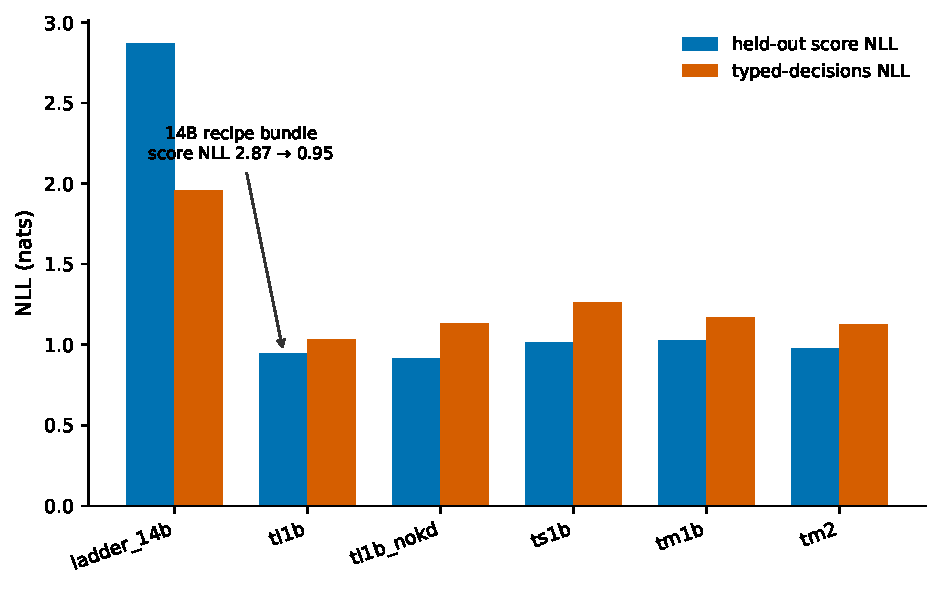
\includegraphics[width=0.6\linewidth]{figures/fig_calibration.pdf}
  \caption{Held-out Score and typed-decisions NLL (held-out sets, not JevBench). \texttt{ladder\_14b} is
  the 14B under the earlier recipe; \texttt{tl1b} is the same backbone under the recipe bundle of
  \Cref{sec:results:calibration}, and \texttt{tl1b\_nokd} drops distillation from that bundle.
  \texttt{ts1b}, \texttt{tm1b} and \texttt{tm2} are the 1.7B and 4B checkpoints with typed heads and
  DecisionMix.}
  \label{fig:calibration}
\end{figure}

\subsection{Scaling}
\label{sec:results:scaling}

\Cref{tab:headline} and \Cref{fig:ladder} run one recipe at four Qwen3 sizes \citep{yang2025qwen3}
and on Qwen3.5-4B, each beside a frozen control: the same base model, untrained, reading next-token letter logits over the
rendered options with three exemplars.

\begin{table}[t]
  \centering
  \caption{Scaling ladder with frozen controls. JevBench: public 231-id subset, unranked; 95\% intervals
  are cluster bootstraps over the paraphrase group (\Cref{sec:setup:jevbench}). MMLU-$\numcands$:
  MMLU-Pro among-$\numcands$. NLL: held-out Score. ms: research-harness single decision at
  $\numcands{=}2$, one pod and build. Frozen: no training, letter logits, 3 exemplars. Small and medium are the \texttt{typical-small}
  and \texttt{typical-medium} releases. Checkpoints: \texttt{ts1b}, \texttt{ts1c}, \texttt{tm1b},
  \texttt{ladder\_8b}, \texttt{tl1b}, \texttt{tm2}.}
  \label{tab:headline}
  \footnotesize
  \setlength{\tabcolsep}{3pt}
  \begin{tabular}{lccrrrr}
    \toprule
    Model & JevBench std [95\% CI] & JevBench hard [95\% CI] & MMLU-$\numcands$ & $\dqsh$ & NLL & ms \\
    \midrule
    Qwen3-1.7B (small v1) & .694 [.569, .819] & .432 [.342, .523] & .343 & .127 & 1.01 & 45 \\
    % small v2 (ts1c): MMLU/dqsh/NLL read from runs/ts1c/results.json; its CIs and the frozen Qwen3.5-4B CIs
    % recomputed with scripts/jev_ci.py's procedure on guychuk/pcdm-runs artefacts (not in prose sources).
    \quad small v2 & .708 [.569, .833] & .432 [.342, .523] & .338 & .127 & 1.08 & -- \\
    \quad frozen, 3-shot & .528 [.389, .667] & .369 [.279, .459] & -- & -- & -- & -- \\
    Qwen3-4B (medium v1) & .806 [.694, .903] & .423 [.333, .514] & .458 & .193 & 1.03 & 57 \\
    \quad frozen, 3-shot & .778 [.667, .889] & .441 [.351, .532] & -- & -- & -- & -- \\
    Qwen3-8B & .667 [.528, .792] & .396 [.306, .486] & .302 & .093 & 1.67 & 70 \\
    \quad frozen, 3-shot & .556 [.417, .694] & .369 [.279, .459] & -- & -- & -- & -- \\
    Qwen3-14B & \textbf{.931} [.861, .986] & .450 [.360, .541] & \textbf{.498} & \textbf{.235} & \textbf{0.95} & 59 \\
    \quad frozen, 3-shot & .819 [.708, .917] & .559 [.468, .649] & -- & -- & -- & -- \\
    Qwen3.5-4B (medium v2) & .861 [.778, .944] & .495 [.405, .586] & .429 & .194 & 0.97 & -- \\
    \quad frozen, 3-shot & .764 [.639, .875] & .495 [.405, .586] & -- & -- & -- & -- \\
    \bottomrule
  \end{tabular}
\end{table}

\begin{figure}[t]
  \centering
  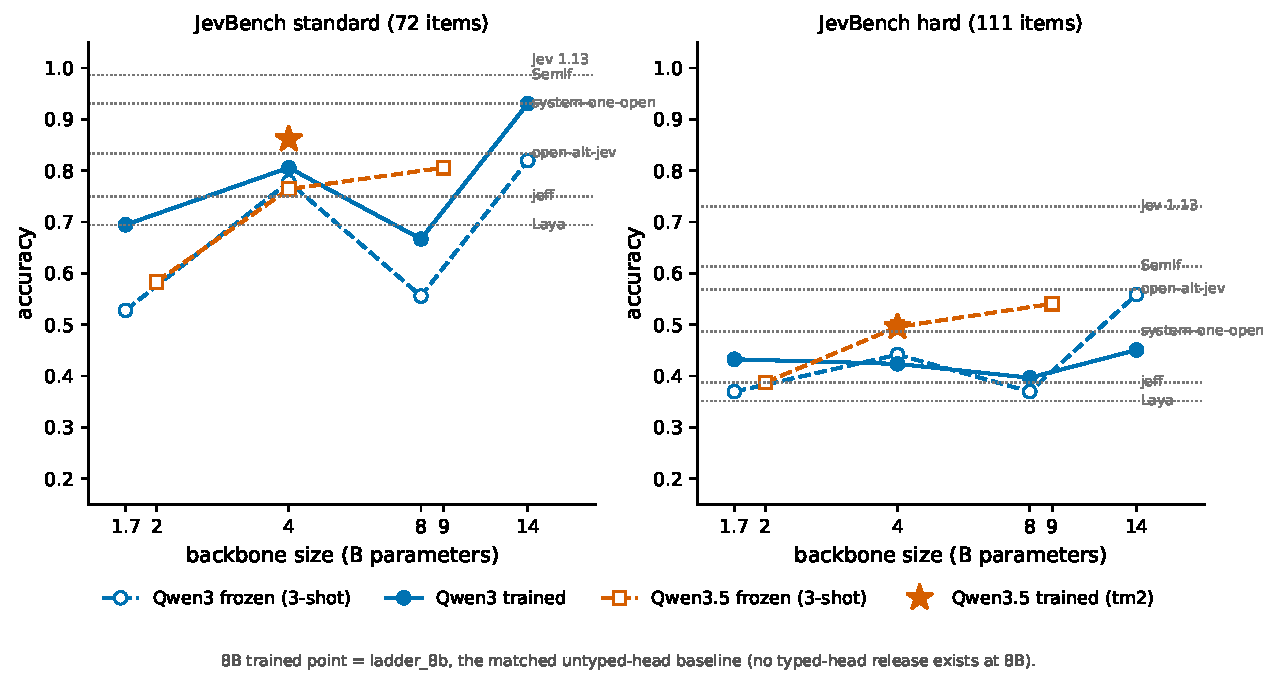
\includegraphics[width=0.9\linewidth]{figures/fig_ladder.pdf}
  \caption{JevBench standard and hard accuracy against backbone size, public 231-id subset, unranked.
  Qwen3 trained (solid) and frozen with three exemplars (dashed); Qwen3.5 frozen controls at 2B/4B/9B and
  the trained Qwen3.5-4B (star). Dotted lines mark other public entries on the same ids, whose rendering
  and protocols differ (\Cref{app:leaderboard}). Intervals are in \Cref{tab:headline}.}
  \label{fig:ladder}
\end{figure}

\textbf{Training beats the frozen backbone on the standard tier at every Qwen3 rung}, by 16.6, 2.8, 11.1
and 11.2 points at 1.7B, 4B, 8B and 14B. The sign is consistent across all four rungs; each gap on its
own sits inside its interval, and the paired test at 14B gives frozen-minus-trained $-.111$
$[-.250, +.014]$, $p = .10$. The 14B checkpoint reaches .931 on the standard tier. Question-conditioned
knowledge grows with the backbone: $\dqsh$ rises from .127 at 1.7B to .193 at 4B and .235 at 14B, 2.3
times the 1.7B teacher's. The second-generation backbone is the strongest point per parameter:
Qwen3.5-4B, released as \texttt{typical-medium} v2, scores .861 standard and .495 hard, above every
Qwen3 checkpoint we trained on the hard tier, and 9.7 standard-tier points above its own frozen control.
The Qwen3-8B rung underperforms its neighbours in both frozen and trained form under the identical
recipe, which marks it as a property of that checkpoint. The hard tier, where the frozen 14B leads, is
discussed in \Cref{sec:limitations}.

\subsection{Cost}
\label{sec:results:cost}

\textbf{Decision latency is nearly flat in backbone size.} On the research harness a single decision at
$\numcands{=}2$ costs 45, 57 and 59\,ms at 1.7B, 4B and 14B: an $8\times$ larger backbone is $1.3\times$
slower, because the cached state and a short suffix dominate. The cost stays flat to $\numcands{=}32$
(46, 58 and 62\,ms) and reaches 106\,ms at 1.7B and 156\,ms at 14B at $\numcands{=}256$. For $M$
questions against one cached state the cost is $O(|\state|) + M \cdot O(|\query| + |\cands|)$, so the
batched marginal cost per question grows with size and candidate tokens: 2.7 and 3.9\,ms at
$\numcands{=}2$ for 1.7B and 14B, 28.0 and 109.7\,ms at $\numcands{=}256$.

\textbf{On the optimized serving path a warm decision takes 15.5--17\,ms at 1.7B.} The released
inference package originally deep-copied the prefix key-value cache on every decision. A zero-copy
strided view, with bit-identical output, plus cached masks and position tensors brings warm p50 from
21--25 to 15.5--17\,ms at 1.7B and from 26--27 to 19--21\,ms for the Qwen3-4B model
(\Cref{fig:serving}); the Qwen3.5-4B model measures 34--46\,ms with reference DeltaNet kernels.

\textbf{Large candidate sets go through a shortlist.} With 256 questions against one state, the
contextual readout's per-question cost grows from 1.07\,ms at $\numcands{=}2$ to 43.8\,ms at
$\numcands{=}256$, while a candidate-blind scorer stays at 0.97--1.06\,ms. Sets in the hundreds are
served by that scorer producing a bounded shortlist for the contextual readout to decide, the role left
to the candidate-blind state of \Cref{sec:analysis:deltaq}, since shortlisting runs on priors.

\subsection{Evidence placement in long states}
\label{sec:results:long}

\textbf{Training with the evidence placed first adds 11.2 points on held-out long states, isolated by a
render-crossed design and replicated at a second seed.} The original long-state workflow corpus rendered
the case facts after the policy text, and the loader right-truncated states to the training window: at
the 1{,}024-token window used for the first releases, 98.8\% of long-policy rows lost their facts
(\Cref{sec:train:long}). Two 1.7B arms with byte-identical flags train on the same 23{,}318 rows, rendered facts-first or
facts-last, with truncation active as at release. Both are scored on 605 held-out long states under both
renders with no truncation at evaluation (4{,}096-token window; state p50 1{,}965 tokens, max 2{,}843).
Matched cells measure what training cost; off-diagonal cells measure render mismatch
(\Cref{tab:twobytwo}).

\begin{table}[t]
  \centering
  \caption{Training render $\times$ evaluation render on 605 held-out long states, no truncation at
  evaluation. Diagonal cells are matched; the matched-vs-matched comparison isolates the training
  effect. Majority floors: \texttt{policy\_permit} .612 ($\numcands{=}2$, $n{=}330$),
  \texttt{action\_select} .233 ($\numcands{=}4$, $n{=}275$). 14B arms: \texttt{tl1b\_nokd}
  (facts-first) and \texttt{ladder\_14b} (facts-last).}
  \label{tab:twobytwo}
  \small
  \setlength{\tabcolsep}{5pt}
  \begin{tabular}{llrrr}
    \toprule
    Trained on & Scored on & overall & \texttt{policy\_permit} & \texttt{action\_select} \\
    \midrule
    \multicolumn{5}{l}{\emph{1.7B, single-variable arms}} \\
    facts-first & facts-first \emph{(matched)} & \textbf{.942} & \textbf{.933} & \textbf{.953} \\
    facts-first & facts-last & .797 & .788 & .807 \\
    facts-last & facts-first & .640 & .615 & .669 \\
    facts-last & facts-last \emph{(matched)} & .830 & .842 & .815 \\
    \midrule
    \multicolumn{5}{l}{\emph{14B corroboration}} \\
    facts-first & facts-first \emph{(matched)} & \textbf{.997} & .997 & .996 \\
    facts-first & facts-last & .921 & .933 & .905 \\
    facts-last & facts-first & .851 & .839 & .865 \\
    facts-last & facts-last \emph{(matched)} & .919 & .930 & .905 \\
    \bottomrule
  \end{tabular}
\end{table}

At 1.7B the matched-condition gap is $+.112$ $[+.077, +.147]$, $p = 5\times10^{-10}$ (\texttt{policy\_permit}
$+.091$ $[+.043, +.139]$, \texttt{action\_select} $+.138$ $[+.086, +.190]$), and a second seed of the
whole pair gives $+.111$. At 14B the gap is $+.078$ $[+.055, +.100]$, $p = 7\times10^{-12}$, smaller
because the facts-first model is at ceiling (.997). The two 14B checkpoints differ in the rest of the
recipe bundle as well, so the 14B pair corroborates the direction and size at scale and the 1.7B pair is
the single-variable test.

\textbf{The fixed checkpoints are the current releases.} With the case facts before the policy body, the
first releases scored .598 (1.7B) and .612 (4B), and on the yes/no family they sat at or below its .612
majority floor (.536 and .555). The v2 releases, trained on the fixed corpus, score .947 and .950
(\texttt{policy\_permit} .948 and .967), and hold their facts-last accuracy (.790 vs.\ .798 at 1.7B, .879
vs.\ .866 at 4B). JevBench does not register the change: \texttt{typical-small} v2 and v1 read
.708 and .694 on its standard tier (\Cref{tab:headline}). The benchmark's 19-item \texttt{long\_policy}
cell could not resolve the effect either, returning $p = .232$ at one seed and a tie at the other
(\Cref{app:hard-tier}).

\subsection{Rendering as an experimental factor}
\label{sec:results:rendering}

\textbf{Changing only the rendering moves a frozen 9B model 12.5 points.} Scoring identical public
JevBench items with identical frozen Qwen3.5 checkpoints and the same letter-logit readout, changing only
the layout of the state and options to a replication of another published system's format, lifts the
standard tier by 1.4, 8.3 and 12.5 points at 2B, 4B and 9B (\Cref{tab:rendering}). The effect survives a
paired per-item test at 4B ($p = .048$) and 9B ($p < .001$), and no hard-tier change separates at any
size.

\begin{table}[t]
  \centering
  \caption{Rendering alone, frozen weights. Identical Qwen3.5 base checkpoints and items (JevBench,
  public 231-id subset, unranked), letter-logit readout in both columns; only the state and option
  rendering differs. $\Delta$: paired cluster bootstrap over the per-item difference, 20{,}000 resamples.}
  \label{tab:rendering}
  \small
  \begin{tabular}{llccc}
    \toprule
    Tier & Backbone & our rendering & replicated rendering & paired $\Delta$ [95\% CI], $p$ \\
    \midrule
    \multirow{3}{*}{standard} & Qwen3.5-2B & .583 & .597 & $+.014$ $[-.194, +.208]$, $p{=}.95$ \\
     & Qwen3.5-4B & .764 & .847 & $+.083$ $[+.014, +.167]$, $p{=}.048$ \\
     & Qwen3.5-9B & .806 & \textbf{.931} & $\mathbf{+.125}$ $[+.056, +.208]$, $p{<}.001$ \\
    \midrule
    \multirow{3}{*}{hard} & Qwen3.5-2B & .387 & .441 & $+.054$ $[-.045, +.153]$, $p{=}.33$ \\
     & Qwen3.5-4B & .495 & .468 & $-.027$ $[-.117, +.063]$, $p{=}.64$ \\
     & Qwen3.5-9B & .541 & .595 & $+.054$ $[-.027, +.135]$, $p{=}.22$ \\
    \bottomrule
  \end{tabular}
\end{table}

\textbf{Inside one trained model, render mismatch costs more than the data defect.} In the off-diagonal
cells of \Cref{tab:twobytwo}, where the evidence is fully visible and only its position changes,
switching the evaluation render against the training render costs 14.5 points for the facts-first 1.7B
model and 19.0 for the facts-last one, which lands on its majority floor on \texttt{policy\_permit}
(.615 against .612). At 14B the same switch costs 7.6 and 6.8 points, so capacity buys render
tolerance that the 1.7B pair alone would not reveal. Our own checkpoints give the sharpest illustration:
the earlier-recipe 14B scores .053 on JevBench's 19-item \texttt{long\_policy} family and .919 on the 605
held-out long states in its own training render. The pair also changes the item set, and the gap
compounds truncation damage, render mismatch against the benchmark's fixed format and a 19-item sample.

A benchmark score therefore measures capability jointly with interface compatibility, and we read our
own numbers that way. The frozen controls of \Cref{tab:headline} use a letter-logit rendering we did not
sweep and the trained models the native one, so frozen-versus-trained comparisons carry a rendering factor
of the size shown here; leaderboard context sits in \Cref{app:leaderboard} for the same reason.
